\documentclass{standalone}
\usepackage{tikz}
\usetikzlibrary{patterns, positioning}

\begin{document}
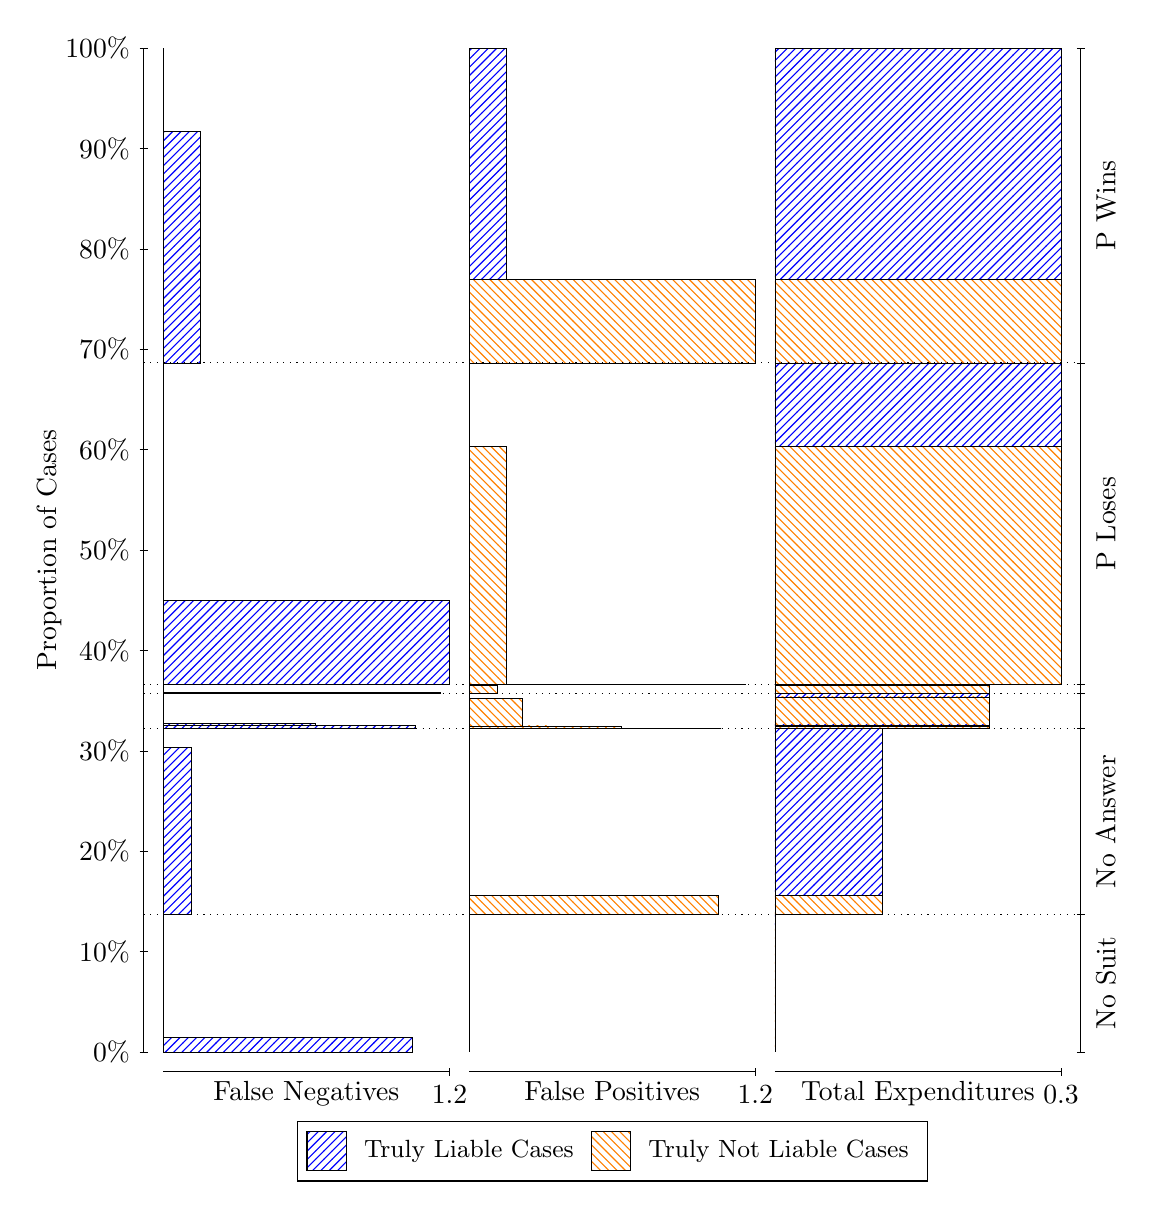
\begin{tikzpicture}
\draw[black, very thin] (1.5,1.75) -- (1.5,14.5);
\node[rotate=90, anchor=center] at (0.3, 8.125) {Proportion of Cases};
\draw[black, very thin] (1.45,1.75) -- (1.55,1.75);
\node[anchor=east] at (1.45, 1.75) {0\%};
\draw[black, very thin] (1.45,3.025) -- (1.55,3.025);
\node[anchor=east] at (1.45, 3.025) {10\%};
\draw[black, very thin] (1.45,4.3) -- (1.55,4.3);
\node[anchor=east] at (1.45, 4.3) {20\%};
\draw[black, very thin] (1.45,5.575) -- (1.55,5.575);
\node[anchor=east] at (1.45, 5.575) {30\%};
\draw[black, very thin] (1.45,6.85) -- (1.55,6.85);
\node[anchor=east] at (1.45, 6.85) {40\%};
\draw[black, very thin] (1.45,8.125) -- (1.55,8.125);
\node[anchor=east] at (1.45, 8.125) {50\%};
\draw[black, very thin] (1.45,9.4) -- (1.55,9.4);
\node[anchor=east] at (1.45, 9.4) {60\%};
\draw[black, very thin] (1.45,10.675) -- (1.55,10.675);
\node[anchor=east] at (1.45, 10.675) {70\%};
\draw[black, very thin] (1.45,11.95) -- (1.55,11.95);
\node[anchor=east] at (1.45, 11.95) {80\%};
\draw[black, very thin] (1.45,13.225) -- (1.55,13.225);
\node[anchor=east] at (1.45, 13.225) {90\%};
\draw[black, very thin] (1.45,14.5) -- (1.55,14.5);
\node[anchor=east] at (1.45, 14.5) {100\%};

\draw[black, very thin] (13.4,1.75) -- (13.4,14.5);
\draw[black, very thin] (13.35,1.75) -- (13.45,1.75);
\node[anchor=west] at (13.35, 1.75) {};
\draw[black, very thin] (13.35,3.4972) -- (13.45,3.4972);
\node[anchor=west] at (13.35, 3.4972) {};
\draw[black, very thin] (13.35,5.8568) -- (13.45,5.8568);
\node[anchor=west] at (13.35, 5.8568) {};
\draw[black, very thin] (13.35,6.3016) -- (13.45,6.3016);
\node[anchor=west] at (13.35, 6.3016) {};
\draw[black, very thin] (13.35,6.418) -- (13.45,6.418);
\node[anchor=west] at (13.35, 6.418) {};
\draw[black, very thin] (13.35,6.418) -- (13.45,6.418);
\node[anchor=west] at (13.35, 6.418) {};
\draw[black, very thin] (13.35,10.502) -- (13.45,10.502);
\node[anchor=west] at (13.35, 10.502) {};
\draw[black, very thin] (13.35,14.5) -- (13.45,14.5);
\node[anchor=west] at (13.35, 14.5) {};

\draw[black, very thin, pattern color=blue, pattern=north east lines] (1.75,1.75) rectangle (4.9094,1.9338);
\draw[black, very thin, pattern color=orange, pattern=north west lines] (1.75,1.9338) rectangle (1.75,3.4972);
\draw[black, very thin, pattern color=blue, pattern=north east lines] (1.75,3.4972) rectangle (2.1054,5.6136);
\draw[black, very thin, pattern color=orange, pattern=north west lines] (1.75,5.6136) rectangle (1.75,5.8568);
\draw[black, very thin, pattern color=blue, pattern=north east lines] (1.75,5.8568) rectangle (4.9489,5.8936);
\draw[black, very thin, pattern color=blue, pattern=north east lines] (1.75,5.8936) rectangle (4.633,5.8954);
\draw[black, very thin, pattern color=blue, pattern=north east lines] (1.75,5.8954) rectangle (4.317,5.8975);
\draw[black, very thin, pattern color=blue, pattern=north east lines] (1.75,5.8975) rectangle (4.0011,5.8975);
\draw[black, very thin, pattern color=blue, pattern=north east lines] (1.75,5.8975) rectangle (4.0011,5.8977);
\draw[black, very thin, pattern color=blue, pattern=north east lines] (1.75,5.8977) rectangle (3.6851,5.9217);
\draw[black, very thin, pattern color=blue, pattern=north east lines] (1.75,5.9217) rectangle (3.3692,5.9217);
\draw[black, very thin, pattern color=blue, pattern=north east lines] (1.75,5.9217) rectangle (3.0533,5.9217);
\draw[black, very thin, pattern color=blue, pattern=north east lines] (1.75,5.9217) rectangle (2.7373,5.9217);
\draw[black, very thin, pattern color=blue, pattern=north east lines] (1.75,5.9217) rectangle (2.4214,5.9217);
\draw[black, very thin, pattern color=orange, pattern=north west lines] (1.75,5.9217) rectangle (1.75,6.3016);
\draw[black, very thin, pattern color=blue, pattern=north east lines] (1.75,6.3016) rectangle (5.2649,6.3132);
\draw[black, very thin, pattern color=orange, pattern=north west lines] (1.75,6.3132) rectangle (1.75,6.418);
\draw[black, very thin, pattern color=blue, pattern=north east lines] (1.75,6.418) rectangle (2.1054,6.418);
\draw[black, very thin, pattern color=orange, pattern=north west lines] (1.75,6.418) rectangle (1.75,6.418);
\draw[black, very thin, pattern color=blue, pattern=north east lines] (1.75,6.418) rectangle (5.3833,7.4807);
\draw[black, very thin, pattern color=orange, pattern=north west lines] (1.75,7.4807) rectangle (1.75,10.502);
\draw[black, very thin, pattern color=blue, pattern=north east lines] (1.75,10.502) rectangle (2.2239,13.438);
\draw[black, very thin, pattern color=orange, pattern=north west lines] (1.75,13.438) rectangle (1.75,14.5);
\draw[black, very thin, pattern color=orange, pattern=north west lines] (5.6333,1.75) rectangle (5.6333,3.3134);
\draw[black, very thin, pattern color=blue, pattern=north east lines] (5.6333,3.3134) rectangle (5.6333,3.4972);
\draw[black, very thin, pattern color=orange, pattern=north west lines] (5.6333,3.4972) rectangle (8.7928,3.7405);
\draw[black, very thin, pattern color=blue, pattern=north east lines] (5.6333,3.7405) rectangle (5.6333,5.8568);
\draw[black, very thin, pattern color=orange, pattern=north west lines] (5.6333,5.8568) rectangle (8.8322,5.8568);
\draw[black, very thin, pattern color=orange, pattern=north west lines] (5.6333,5.8568) rectangle (8.5163,5.8568);
\draw[black, very thin, pattern color=orange, pattern=north west lines] (5.6333,5.8568) rectangle (8.2004,5.8568);
\draw[black, very thin, pattern color=orange, pattern=north west lines] (5.6333,5.8568) rectangle (7.8844,5.8568);
\draw[black, very thin, pattern color=orange, pattern=north west lines] (5.6333,5.8568) rectangle (7.5685,5.8811);
\draw[black, very thin, pattern color=orange, pattern=north west lines] (5.6333,5.8811) rectangle (7.2525,5.8816);
\draw[black, very thin, pattern color=orange, pattern=north west lines] (5.6333,5.8816) rectangle (6.9366,5.8864);
\draw[black, very thin, pattern color=orange, pattern=north west lines] (5.6333,5.8864) rectangle (6.6207,5.8924);
\draw[black, very thin, pattern color=orange, pattern=north west lines] (5.6333,5.8924) rectangle (6.3047,6.2367);
\draw[black, very thin, pattern color=blue, pattern=north east lines] (5.6333,6.2367) rectangle (5.6728,6.2367);
\draw[black, very thin, pattern color=blue, pattern=north east lines] (5.6333,6.2367) rectangle (5.6333,6.3016);
\draw[black, very thin, pattern color=orange, pattern=north west lines] (5.6333,6.3016) rectangle (5.9888,6.4063);
\draw[black, very thin, pattern color=blue, pattern=north east lines] (5.6333,6.4063) rectangle (5.6333,6.418);
\draw[black, very thin, pattern color=orange, pattern=north west lines] (5.6333,6.418) rectangle (9.1482,6.418);
\draw[black, very thin, pattern color=blue, pattern=north east lines] (5.6333,6.418) rectangle (5.9888,6.418);
\draw[black, very thin, pattern color=orange, pattern=north west lines] (5.6333,6.418) rectangle (6.1072,9.4396);
\draw[black, very thin, pattern color=blue, pattern=north east lines] (5.6333,9.4396) rectangle (5.6333,10.502);
\draw[black, very thin, pattern color=orange, pattern=north west lines] (5.6333,10.502) rectangle (9.2667,11.564);
\draw[black, very thin, pattern color=blue, pattern=north east lines] (5.6333,11.564) rectangle (6.1072,14.5);
\draw[black, very thin, pattern color=orange, pattern=north west lines] (9.5167,1.75) rectangle (9.5167,3.3134);
\draw[black, very thin, pattern color=blue, pattern=north east lines] (9.5167,3.3134) rectangle (9.5167,3.4972);
\draw[black, very thin, pattern color=orange, pattern=north west lines] (9.5167,3.4972) rectangle (10.879,3.7405);
\draw[black, very thin, pattern color=blue, pattern=north east lines] (9.5167,3.7405) rectangle (10.879,5.8568);
\draw[black, very thin, pattern color=orange, pattern=north west lines] (9.5167,5.8568) rectangle (12.242,5.8568);
\draw[black, very thin, pattern color=blue, pattern=north east lines] (9.5167,5.8568) rectangle (12.242,5.8568);
\draw[black, very thin, pattern color=orange, pattern=north west lines] (9.5167,5.8568) rectangle (12.242,5.8811);
\draw[black, very thin, pattern color=blue, pattern=north east lines] (9.5167,5.8811) rectangle (12.242,5.905);
\draw[black, very thin, pattern color=orange, pattern=north west lines] (9.5167,5.905) rectangle (12.242,6.2601);
\draw[black, very thin, pattern color=blue, pattern=north east lines] (9.5167,6.2601) rectangle (12.242,6.3007);
\draw[black, very thin, pattern color=orange, pattern=north west lines] (9.5167,6.3007) rectangle (12.242,6.3013);
\draw[black, very thin, pattern color=blue, pattern=north east lines] (9.5167,6.3013) rectangle (12.242,6.3016);
\draw[black, very thin, pattern color=orange, pattern=north west lines] (9.5167,6.3016) rectangle (12.242,6.3016);
\draw[black, very thin, pattern color=blue, pattern=north east lines] (9.5167,6.3016) rectangle (12.242,6.3016);
\draw[black, very thin, pattern color=orange, pattern=north west lines] (9.5167,6.3016) rectangle (12.242,6.4063);
\draw[black, very thin, pattern color=blue, pattern=north east lines] (9.5167,6.4063) rectangle (12.242,6.418);
\draw[black, very thin, pattern color=orange, pattern=north west lines] (9.5167,6.418) rectangle (12.242,6.418);
\draw[black, very thin, pattern color=blue, pattern=north east lines] (9.5167,6.418) rectangle (12.242,6.418);
\draw[black, very thin, pattern color=orange, pattern=north west lines] (9.5167,6.418) rectangle (13.15,9.4396);
\draw[black, very thin, pattern color=blue, pattern=north east lines] (9.5167,9.4396) rectangle (13.15,10.502);
\draw[black, very thin, pattern color=orange, pattern=north west lines] (9.5167,10.502) rectangle (13.15,11.564);
\draw[black, very thin, pattern color=blue, pattern=north east lines] (9.5167,11.564) rectangle (13.15,14.5);
\draw[black, dotted] (1.5,3.4972) -- (13.4,3.4972);
\draw[black, dotted] (1.5,5.8568) -- (13.4,5.8568);
\draw[black, dotted] (1.5,6.3016) -- (13.4,6.3016);
\draw[black, dotted] (1.5,6.418) -- (13.4,6.418);
\draw[black, dotted] (1.5,6.418) -- (13.4,6.418);
\draw[black, dotted] (1.5,10.502) -- (13.4,10.502);
\draw[black, very thin] (1.75,1.5) -- (5.3833,1.5);
\node[anchor=north] at (3.5667, 1.5) {False Negatives};
\draw[black, very thin] (5.3833,1.45) -- (5.3833,1.55);
\node[anchor=north] at (5.3833, 1.45) {1.2};

\draw[black, very thin] (5.6333,1.5) -- (9.2667,1.5);
\node[anchor=north] at (7.45, 1.5) {False Positives};
\draw[black, very thin] (9.2667,1.45) -- (9.2667,1.55);
\node[anchor=north] at (9.2667, 1.45) {1.2};

\draw[black, very thin] (9.5167,1.5) -- (13.15,1.5);
\node[anchor=north] at (11.333, 1.5) {Total Expenditures};
\draw[black, very thin] (13.15,1.45) -- (13.15,1.55);
\node[anchor=north] at (13.15, 1.45) {0.3};

\node[black, centered, rotate=90] at (13.72, 2.6236) {No Suit};
\node[black, centered, rotate=90] at (13.72, 4.677) {No Answer};



\node[black, centered, rotate=90] at (13.72, 8.4601) {P Loses};
\node[black, centered, rotate=90] at (13.72, 12.501) {P Wins};

\draw (7.449999999999999,1.5) node[draw=none] (baseCoordinate) {};
\begin{scope}[align=center]
        \matrix[scale=0.5, draw=black, below=0.5cm of baseCoordinate, nodes={draw}, column sep=0.1cm]{
            \node[rectangle, draw, minimum width=0.5cm, minimum height=0.5cm, pattern=north east lines, pattern color=blue] {}; &
            \node[draw=none, font=\small] (B) {Truly Liable Cases}; &
            \node[rectangle, draw, minimum width=0.5cm, minimum height=0.5cm, pattern=north west lines, pattern color=orange] {}; &
            \node[draw=none, font=\small] (B) {Truly Not Liable Cases}; \\
            };
\end{scope}

\end{tikzpicture}
\end{document}